\documentclass[journal]{IEEEtran}

\usepackage{amsmath,amssymb}
\usepackage{booktabs}
\usepackage{graphicx}
\usepackage{multirow}
\usepackage{cite}
\usepackage{url}
\usepackage{xcolor}

\graphicspath{{./}}
\newcommand{\method}{HTA-MAC}
\newcommand{\E}{\mathbb{E}}
\newcommand{\R}{\mathbb{R}}
\newcommand{\ind}{\mathbb{I}}

\begin{document}

\title{HTA-MAC: Permutation-Equivariant Distributional Scheduling for Clustered Energy-Harvesting Sensor Networks}

\author{Anonymous Authors}

\maketitle

\begin{abstract}
Energy-harvesting wireless sensor networks require a medium-access controller
to use intermittent energy without exhausting vulnerable relays or allowing
queued measurements to expire. Fixed time-division schedules do not resolve
this tradeoff, while a direct joint action over all cluster members grows
exponentially. This paper presents \method, a cluster-level scheduler that
assigns zero to three transmission slots per member under a hard frame budget.
Its distributional branching network shares the same node encoder and action
head across members, uses permutation-invariant set context, and projects
marginal action values onto the feasible budget. The state combines residual
energy, queue age, harvest forecasts, and scheduled-cluster-head risk without
changing cluster-head selection or routing. Evaluation across paired traffic,
energy, topology, and trace-replay conditions shows that \method{} produces
exactly feasible actions, lowers stale loss, and improves service fairness over
energy-proportional allocation in medium and large networks. The architecture
is evaluated through 300 nodes while retaining constant learned parameter
storage. Aggregate delivery, energy efficiency, and first-death
lifetime remain stronger for the best matched baselines, exposing a clear
fairness--staleness versus service-volume tradeoff. These findings position
\method{} as a scalable and auditable learned scheduling architecture rather
than a universal replacement for analytical allocation rules, and identify
the policy improvements required before independent deployment validation.
\end{abstract}

\begin{IEEEkeywords}
energy harvesting, wireless sensor networks, medium access control,
distributional reinforcement learning, TDMA, constrained scheduling.
\end{IEEEkeywords}

\section{Introduction}

\IEEEPARstart{E}{nergy-harvesting} wireless sensor networks (EH-WSNs) replace
a fixed energy budget with a stochastic one. The resulting design objective is
not simply to postpone battery exhaustion. A conservative node may survive
while measurements expire in its queue; an aggressive node may deliver more
traffic while accelerating the first network death. Iannello \emph{et al.}
therefore framed EH medium access through a delivery--efficiency tradeoff
rather than lifetime alone \cite{iannello2012ehmac}. That distinction remains
central when a clustered network adds a second energy bottleneck: every packet
served within a cluster also creates reception, aggregation, and long-range
forwarding work at the scheduled cluster head (CH).

TDMA is attractive in this setting because it avoids contention and permits
sleeping outside assigned slots. Yet equal or fixed assignment wastes channel
time when queues and harvested energy differ. Forecast-aware assignment
methods improve utilization \cite{gong2021ffss}, while adaptive EH protocols
adjust duty cycle, contention, or cross-layer operation
\cite{movva2022s2a2mac,sarang2024henomac,lee2021reemac,sefuba2015adaptive}.
These approaches motivate adaptation, but do not by themselves solve the
coupled per-member allocation problem under a shared frame budget.

Reinforcement learning (RL) offers a state-conditioned alternative.
Cooperative and deep RL have been used for solar-powered throughput
\cite{ge2021cooperative,hasani2025drl}, energy-aware multi-access
\cite{chu2019multiaccess}, delay-sensitive sensing \cite{sharma2019structure},
and adaptive underwater TDMA \cite{eris2024underwaterrl}. A naive discrete
formulation nevertheless has $(n_{\max}+1)^m$ joint actions for $m$ members and
$n_{\max}$ slots per member. Independent heads avoid this explosion but can
encode branch identity and fail when membership or node order changes. They
also need a mechanism that enforces the cluster budget exactly.

This paper addresses these issues at the intra-cluster MAC layer. The CH
schedule, member association, and inter-cluster forwarding rule are treated as
exogenous. This boundary isolates a testable question: given the scheduled CH
and current cluster state, which members should transmit, and how many queued
packets should each send? Fig.~\ref{fig:architecture} summarizes the resulting
shared-parameter scheduling path.

\begin{figure}[t]
  \centering
  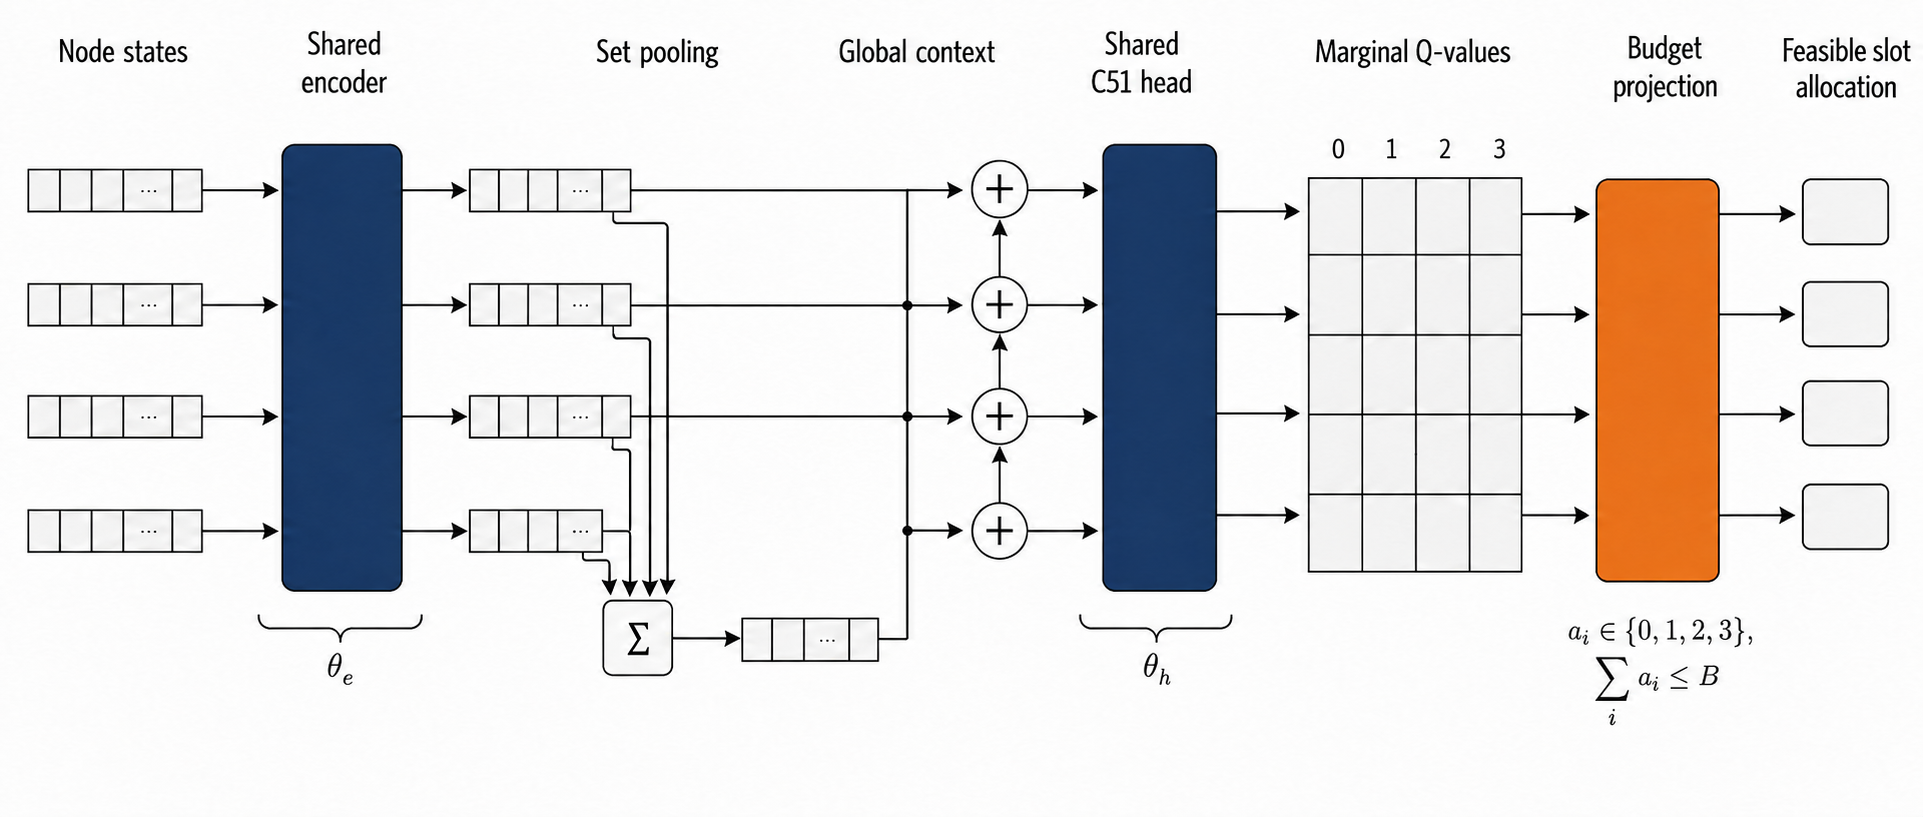
\includegraphics[width=\columnwidth]{hta_mac_architecture.png}
  \caption{\method{} architecture. Shared node encoding and invariant set
  context produce marginal action values, which are projected onto the hard
  slot budget.}
  \label{fig:architecture}
\end{figure}

The contributions are threefold.

\begin{itemize}
\item We formulate budgeted per-node TDMA with queue age, idle listening,
stochastic harvesting, and CH-role energy, and distinguish service, fairness,
efficiency, and survival.
\item We develop permutation-equivariant distributional branching. Shared set
processing removes node identity; marginal-value projection guarantees
feasibility.
\item We evaluate 20 independent paired realizations across ten transfer
conditions using bootstrap intervals, signed-rank tests, and multiplicity
correction, then use a separate simultaneous-all-cluster pilot to quantify
fair-energy retention under increased traffic; node-count scaling, component
interventions, parameter memory, and decision latency are reported separately.
\end{itemize}

The evidence supports a deliberately bounded conclusion. \method{} provides
exact feasible learned allocation with constant learned parameter storage and
meaningful stale-loss/fairness behavior, but cap-corrected energy allocation
and online primal--dual are stronger on service volume and lifetime. The
contribution is architectural and diagnostic, not a superiority claim.

\section{Related Work}

\subsection{Energy-Harvesting Medium Access}

Analytical EH-MAC work established that reliable delivery and time efficiency
must be considered jointly \cite{iannello2012ehmac}. Forecast-aware TDMA later
cast slot assignment and frame sizing as polynomial optimization problems,
showing that upcoming data and energy can reduce empty slots
\cite{gong2021ffss}. Predictive solar control has also been evaluated with
measured harvesting sequences and small-scale experiments
\cite{zou2016predictive}. These studies provide the metric and validation
foundations for the present work, but they do not learn a variable-cardinality
per-member allocation policy.

Energy-efficient wireless control commonly measures reliable goodput per
joule while imposing delay or statistical QoS constraints
\cite{meshkati2007energy,gao2017statistical}. Fair resource allocation exposes
the accompanying sum-service tradeoff through $\alpha$-fair utility or Jain's
index \cite{yang2018fairness,jain1984fairness}. Because energy, robustness,
and delay can be antagonistic, multiobjective wireless evaluation favors
Pareto tradeoffs over an opaque weighted leaderboard
\cite{jaffres2010multiobjective}. These principles motivate the secondary
fair-energy and load-retention endpoints introduced below; they do not replace
the component metrics.

Clustered protocols couple channel access to routing, sink placement, or CH
selection. S2A2MAC combines energy-aware clustering and semi-synchronized
access \cite{movva2022s2a2mac}; adaptive cross-layer scheduling jointly uses
application and MAC information \cite{sefuba2015adaptive}; REE-MAC estimates
residual energy in wireless-powered networks \cite{lee2021reemac}; and
HENO-MAC adjusts duty cycle using solar--wind energy-neutral conditions
\cite{sarang2024henomac}. Their broader scope is complementary. Here, the CH
schedule is held fixed so that observed effects are attributable to
member-slot allocation.

\subsection{Learning-Based Scheduling}

RL has been applied to decentralized EH access, prediction, sensing, and
fairness \cite{chu2019multiaccess,sharma2019structure,li2018fair,
biason2016decentralized,leong2020drl}. In clustered solar networks, cooperative
Q-learning balances consumption and harvesting \cite{ge2021cooperative}; a
recent DQN study uses continuous energy states to improve throughput
\cite{hasani2025drl}. The closest action-level analogue is harvesting-aware
underwater TDMA, where individual agents learn transmission slots and the
authors report FND, HND, and LND \cite{eris2024underwaterrl}. Its underwater
channel, decentralized bandit action, and harvesting objective differ from
the terrestrial queue- and CH-coupled setting considered here.

The present architecture combines three ideas not normally joined in EH-MAC:
categorical return distributions \cite{bellemare2017c51}, action branching
\cite{tavakoli2018branching}, and permutation-invariant set representations
\cite{zaheer2017deepsets}. The combination is functional rather than cosmetic:
distributional values represent heterogeneous long-run outcomes; branching
keeps output growth linear in cluster size; and shared set processing makes
the policy independent of arbitrary member order.

Table~\ref{tab:literature} summarizes the closest methodological neighbors.
The table avoids cross-paper percentage ranking because no two studies share
the same channel, traffic, energy, and survival definitions. It instead shows
the unresolved axis addressed here: centralized multi-packet member allocation
under a hard cluster budget, with permutation-safe generalization and paired
survival-aware inference.

\begin{table*}[t]
\centering
\caption{Positioning Against Closely Related Energy-Harvesting Scheduling Work}
\label{tab:literature}
\scriptsize
\begin{tabular}{@{}p{2.35cm}p{2.15cm}p{3.0cm}p{2.6cm}p{5.2cm}@{}}
\toprule
Study & Network & Adaptive decision & Main evidence & Boundary relative to this work \\
\midrule
Iannello \emph{et al.} \cite{iannello2012ehmac} & Single-hop EH-WSN & TDMA/ALOHA protocol parameters & Analytical delivery--time tradeoff & Establishes tradeoff metrics; no learned clustered allocation. \\
Gong \emph{et al.} \cite{gong2021ffss} & Terrestrial EH-WSN & Slot assignment and frame size & Optimization and simulation & Forecast-aware assignment, but not queue-age/CH-risk RL. \\
Movva \emph{et al.} \cite{movva2022s2a2mac} & Clustered EH-WSN & Clustering, routing, semi-synchronized MAC & End-to-end simulation & Broader network scope; causal MAC effect is not isolated. \\
Ge \emph{et al.} \cite{ge2021cooperative} & Clustered solar WSN & Cooperative transmission rate & Q-learning simulation & Cooperative throughput control without hard branching projection. \\
Hasani \emph{et al.} \cite{hasani2025drl} & Clustered solar WSN & Energy-conditioned transmission action & DQN, node-count sweep & Continuous-state DRL; omits idle energy and paired uncertainty. \\
Eriş \emph{et al.} \cite{eris2024underwaterrl} & Underwater EH-WSN & Decentralized TDMA slot choice & RL, FND/HND/LND & Closest adaptive TDMA analogue; different acoustic channel and action. \\
HENO-MAC \cite{sarang2024henomac} & Hybrid solar--wind IoT & Receiver duty cycle & Real-trace simulation & Strong trace use and delay focus; threshold rather than learned allocation. \\
REE-MAC \cite{lee2021reemac} & Wireless-powered WSN & Access from residual-energy estimate & Protocol simulation & Residual-energy control without stochastic queue/CH-role state. \\
Chu \emph{et al.} \cite{chu2019multiaccess} & EH IoT access & Multi-access and battery prediction & LSTM--DQN simulation & Joint prediction/control, but not clustered budgeted TDMA. \\
Sharma \emph{et al.} \cite{sharma2019structure} & Delay-sensitive EH sensor & Structured transmission policy & Model-based RL analysis & Exploits policy structure; does not address variable-cardinality sets. \\
\method{} & Clustered terrestrial EH-WSN & 0--3 slots per member under $B$ & 20 paired runs, ten transfers & Exogenous CH/routing; one-cluster rank intervention, not end-to-end control. \\
\bottomrule
\end{tabular}
\end{table*}

\section{System Model and Problem Formulation}

\subsection{Clustered Network}

Let $\mathcal{V}=\{1,\ldots,N\}$ denote sensor nodes deployed in a planar
field. At round $t$, an exogenous schedule selects CH set $\mathcal{C}_t$ and
assigns each non-CH node to one CH. For a scheduled cluster $c$, let
$\mathcal{M}_{c,t}$ be its alive members and $m_{c,t}=|\mathcal{M}_{c,t}|$.
The controller selects
\begin{equation}
 a_{i,t}\in\{0,1,\ldots,n_{\max}\},\qquad
 \sum_{i\in\mathcal{M}_{c,t}}a_{i,t}\leq B,
 \label{eq:budget}
\end{equation}
where $a_{i,t}=0$ is a sleep/no-service decision, $n_{\max}=3$, and the frame
budget is $B=24$. A member can serve at most its queue occupancy, so the
delivered packets are $y_{i,t}=\min\{q_{i,t},a_{i,t}\}$.

Packets are retained for at most $L$ rounds and queues hold at most $Q$ packets.
Writing $A_{i,t}$ for new arrivals, $s_{i,t}$ for expiry after service, and
$o_{i,t}$ for overflow, queue evolution is
\begin{equation}
 q_{i,t+1}=\min\!\left\{Q,
 [q_{i,t}-y_{i,t}-s_{i,t}]^{+}+A_{i,t}\right\},
 \label{eq:queue}
\end{equation}
with $L=3$ and $Q=5$. Expiry is tracked from packet ages, rather than inferred
from a terminal backlog.

\subsection{Communication and Energy}

The first-order radio model follows the standard clustered WSN abstraction
\cite{heinzelman2000leach}. For $b$ bits sent over distance $d$,
\begin{equation}
 E_{\mathrm{tx}}(b,d)=
 \begin{cases}
 b(E_{\mathrm{elec}}+\epsilon_{\mathrm{fs}}d^2),&d<d_0,\\
 b(E_{\mathrm{elec}}+\epsilon_{\mathrm{mp}}d^4),&d\ge d_0,
 \end{cases}
 \label{eq:radio}
\end{equation}
where $d_0=\sqrt{\epsilon_{\mathrm{fs}}/\epsilon_{\mathrm{mp}}}$.
Reception and aggregation consume $bE_{\mathrm{elec}}$ and $bE_{\mathrm{DA}}$,
respectively. Each served member transmits its packets to the CH. The CH
receives and aggregates the member payload, then sends one aggregate packet to
the base station. This separates member-transmission cost from CH reception,
aggregation, and forwarding cost.

An awake transmitter listens during the other used slots in its cluster. If
$F_{c,t}=\sum_i a_{i,t}$ is the active frame length, its modeled idle cost is
\begin{equation}
 E^{\mathrm{idle}}_{i,t}=
 (F_{c,t}-a_{i,t})^{+}\,\tau_{\mathrm{slot}}E_{\mathrm{elec}},
 \label{eq:idle}
\end{equation}
where $\tau_{\mathrm{slot}}$ is expressed in bit-time equivalents. Without
this term, a member that stays awake but does not transmit can be energetically
indistinguishable from one that sleeps.

Let $H_{i,t}\ge0$ be harvested energy and $C_{i,t}$ the sum of communication
and idle costs. Stored energy evolves as
\begin{equation}
 E_{i,t+1}=\min\{E_{\max},[E_{i,t}-C_{i,t}]^{+}+H_{i,t}\}.
 \label{eq:battery}
\end{equation}
The controller observes state-conditioned solar and thermal transition
probabilities and rectified next-round moments. The solar model is inherited
from trained upstream parameters; the thermal component is a fixed synthetic
auxiliary and is not represented as measured or trained thermal evidence.

\subsection{Endpoints and Constrained Objective}

For cumulative offered demand $D$, delivery and stale ratios are
\begin{equation}
 \rho_{\mathrm{del}}=\frac{\sum_{i,t}y_{i,t}}{D},\qquad
 \rho_{\mathrm{stale}}=\frac{\sum_{i,t}s_{i,t}}{D}.
 \label{eq:qos}
\end{equation}
Service fairness over member totals $Y_i=\sum_t y_{i,t}$ is Jain's index
\cite{jain1984fairness},
\begin{equation}
 J=\frac{(\sum_iY_i)^2}{m\sum_iY_i^2}.
 \label{eq:jain}
\end{equation}
Energy efficiency is total delivered packets divided by network joules. First
node death (FND) is the first round at which any node has zero stored energy.
For evaluation horizon $T$, restricted survival time is
$\min\{T,T_{\mathrm{FND}}\}$, the single-event analogue of restricted mean
survival time (RMST) \cite{uno2014rmst}. Event counts are reported with it so
censoring cannot be mistaken for failure-free operation.

For scenario $s$ and policy $p$, let $G_{s,p}$ denote successful network
packets and $E_{s,p}^{\mathrm{net}}$ total network energy. We define
Jain-weighted goodput efficiency (JWGE) as
\begin{equation}
 \Gamma_{s,p}=\frac{G_{s,p}}{E_{s,p}^{\mathrm{net}}}J_{s,p},
 \label{eq:jwge}
\end{equation}
which remains in packets/J because $J$ is dimensionless. To measure robustness
to offered load without choosing a scalar weight, the paired load-robust
fair-energy retention (LRFER) for realization $r$ is
\begin{equation}
 R_{r,p}^{\mathrm{load}}=
 \frac{\Gamma_{\mathrm{high},r,p}}
      {\Gamma_{\mathrm{ref},r,p}}.
 \label{eq:lrfer}
\end{equation}
A value of one denotes full retention. Equations~\eqref{eq:jwge}--\eqref{eq:lrfer}
are secondary endpoints: raw packets/J, $J$, delivery, stale loss, and survival
are always reported with them.

The control objective is multi-criteria. During learning, a scalar physical
reward encourages delivered packets, fairness, forecast-aligned service, and
reduced idle energy while penalizing declining-energy allocation, death, and
service through a depleted scheduled CH. QoS constraints impose
\begin{equation}
 \rho_{\mathrm{del}}\ge\delta,\quad
 \rho_{\mathrm{stale}}\le\sigma,\quad J\ge\phi,
 \label{eq:constraints}
\end{equation}
with episode-level dual updates. These constraints guide training; the final
scientific comparison reports all continuous endpoints rather than reducing
them to a binary pass.

\section{HTA-MAC}

\subsection{State and CH-Conditioned Risk}

For every physical node, the observation contains residual energy, one-step
harvest mean and variance, solar and thermal transition rows, normalized queue,
previous allocation, cluster size, packet-age counts, and feasible-action
indicators. A fixed 32-dimensional spatial context is appended. Seven values
describe the scheduled CH and target cluster: CH reserve, forecast and
uncertainty, CH-to-base-station distance, feasible backlog, member fraction,
and CH availability. The resulting per-node vector has 65 features. Broadcast
cluster features enter a shared function and therefore do not provide a node
identifier.

The CH-risk term is activated only below reserve fraction $\eta$. Define
reserve deficit $u_t=[(\eta-E_{c,t}/E_{\max})/\eta]_0^1$, normalized forecast
$h_t$, normalized CH-to-base-station distance $d_t$, and normalized intended
service $\ell_t$. The training penalty is
\begin{equation}
 r_t^{\mathrm{CH}}=-u_t\ell_t(1+w_d d_t)(1-w_h h_t).
 \label{eq:risk}
\end{equation}
It discourages forwarding load specifically when the scheduled CH is depleted,
distant, and unlikely to replenish. It neither observes realized future
harvest nor modifies the CH schedule.

\subsection{Permutation-Equivariant Distributional Branching}

Let $x_i\in\R^p$ be the observation for member $i$ and $m_i\in\{0,1\}$ its
active mask. A shared encoder produces $z_i=f_\theta(x_i)$. Global context is
formed from invariant reductions,
\begin{equation}
 g=\psi_\theta\!\left(
 \frac{\sum_i m_i z_i}{\sum_i m_i},
 \max_{i:m_i=1}z_i,
 \frac{1}{M}\sum_i m_i,
 \frac{B}{M}\right),
 \label{eq:set}
\end{equation}
where $M$ is the padded branch capacity. The same advantage function is applied
to every active node. For categorical atom $k$ and action $a$,
\begin{equation}
 \ell_{i,a,k}=V_k(g)+A_{a,k}(z_i,g)
 -\frac{1}{n_{\max}+1}\sum_{a'}A_{a',k}(z_i,g).
 \label{eq:dueling}
\end{equation}
Softmax probabilities $p_{i,a,k}$ over 51 fixed atoms $\zeta_k\in[-30,30]$
define the branch value
\begin{equation}
 Q_i(a)=\sum_{k=1}^{51}p_{i,a,k}\zeta_k.
 \label{eq:c51}
\end{equation}
Categorical Bellman projection and replay follow C51
\cite{bellemare2017c51}; the branching factorization follows
\cite{tavakoli2018branching}. A development-only return scale keeps targets
inside the fixed support and does not change physical metrics.

For any permutation matrix $P$, shared encoding and invariant pooling give
$Q(PX, Pm)=P Q(X,m)$. Thus permuting node order permutes branch outputs but
does not change their values. Numerical equivariance tests of the implemented
network found maximum absolute expected-value error below
$1.4\times10^{-6}$. Training and evaluation used the same numerical software
configuration.

\subsection{Hard-Budget Projection}

Independent branch maxima need not satisfy \eqref{eq:budget}. For each node,
define the marginal value of its $r$th slot as
\begin{equation}
 \Delta_{i,r}=Q_i(r)-Q_i(r-1),\qquad r=1,\ldots,n_{\max}.
 \label{eq:marginal}
\end{equation}
Starting from zero allocation, the projector repeatedly assigns the currently
largest positive feasible marginal gain until the budget is exhausted or no
positive gain remains. Queue-derived action caps prevent allocation above
available backlog. The procedure is $O(B\log m)$ with a heap, returns an
integer feasible action, and preserves node-permutation equivariance away from
exactly equal marginal values. Exact ties use deterministic branch order; the
equivariance claim therefore applies to the learned value map, not to this
measure-zero tie convention. Fig.~\ref{fig:architecture} summarizes the policy
path.

At deployment, one policy call masks dead, CH, and non-member branches;
computes the shared categorical values; caps each branch by queue-feasible
demand; inserts each branch's first marginal value into a max-priority queue;
and accepts at most $B$ positive increments. After selecting a branch, its next
marginal value is inserted when available. This is not a soft penalty: the
returned action satisfies \eqref{eq:budget} by construction for every state.

\subsection{Model Size and Execution Cost}

With 65 input features, hidden width 128, four actions, and 51 atoms, the
network contains 116,033 trainable parameters. The count is independent of the
number of active members because encoders and advantage heads are shared. In
FP32 the learned parameters occupy 0.443~MiB. For input width $p$, hidden width
$h$, $A$ actions, $K$ atoms, and $m$ active branches, forward inference and
projection require
\begin{equation}
\begin{aligned}
T(m)&=O\!\left(m(ph+h^2+hAK)\right)+O(m+B\log m),\\
M(m)&=O\!\left(P+m(h+AK)\right),
\end{aligned}
\label{eq:complexity}
\end{equation}
where $P$ is the parameter count. The $m$ term in projection builds the heap;
at most $B$ subsequent updates cost $O(\log m)$ each.

Fig.~\ref{fig:complexity} compares exact architectural parameter storage and an
isolated controller microbenchmark. At branch capacity 100, the shared model
remains at 116,033 parameters, versus 3,037,811 for a global encoder with
branch-specific heads and 5,817,700 for independent DQNs. On a single CPU
thread, median neural inference plus projection increased from 0.344~ms at 10
active branches to 0.734~ms at 100; the latter 2.5--97.5 percentile interval
across 30 blocks was 0.672--0.804~ms. Timing is machine-specific and measures
controller computation, not radio or simulator time. This separates
representational capacity from cluster size and supports the same model for
20-, 50-, and 100-node transfer conditions.
The experiments execute inference centrally at the scheduler; they do not
assume that every sensor carries or trains the neural network.

\begin{figure*}[t]
  \centering
  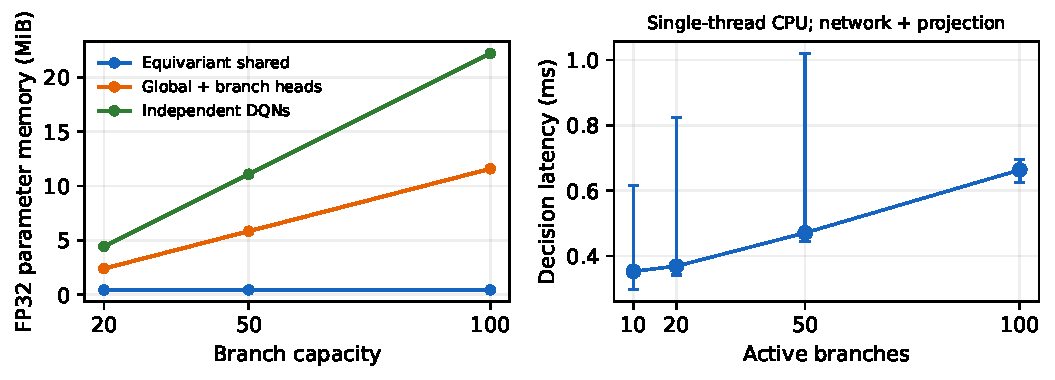
\includegraphics[width=0.88\textwidth]{complexity_profile.pdf}
  \caption{Computational scaling. Left: exact FP32 parameter storage for three
  architectural forms; only the equivariant shared model is branch-capacity
  independent. Right: isolated \method{} inference and budget projection using
  30 blocks of 100 decisions after 100 warm-ups on one CPU thread; bars show
  block-level 2.5--97.5 percentile intervals.}
  \label{fig:complexity}
\end{figure*}

\subsection{Training Procedure}

The reported controller was obtained from one two-stage training pipeline. A
QoS-distilled scheduler first provided the shared representation; the
categorical output layers were then reinitialized and fine-tuned for 100
episodes because the return geometry changed. Training used five independent
network realizations and a curriculum over scheduled CH ranks. The discount
factor was 0.99, batch size 64, and learning rate $10^{-5}$. Exploration
decreased from 1.0 to 0.05. Auxiliary trajectory-order and concavity losses
regularized marginal slot values. Episode-end multipliers used $\delta=0.235$,
$\sigma=0.45$, and $\phi=0.70$.

Hyperparameters and model selection used development realizations only. The 20
independent evaluation realizations were held out until the training procedure
and statistical analysis were finalized.

\section{Experimental Methodology}

\subsection{Environment and Baselines}

The reference network contains 100 nodes uniformly deployed over
$100\times100$~m$^2$, with the base station at $(50,175)$~m. Initial energy is
0.5~J and CH ratio is 0.05. Each data packet has 4000 bits. The radio uses
$E_{\mathrm{elec}}=50$~nJ/bit, $E_{\mathrm{DA}}=5$~nJ/bit,
$\epsilon_{\mathrm{fs}}=10$~pJ/bit/m$^2$, and
$\epsilon_{\mathrm{mp}}=1.3$~fJ/bit/m$^4$. The horizon is 3000 rounds, although
all FND events occur earlier in the reported experiments. Arrivals are
Poisson with reference rate one packet per node per round.

To separate MAC effects from a learned CH selector, evaluation uses an
independently generated balanced rotation. Node positions are redrawn for each
realization; approximately 5\% of nodes are CHs each round; and every node is rotated
through the CH role over an epoch. One rank-specific rollout applies the tested
policy to one scheduled cluster while other clusters use equal allocation.
The inference unit is the run mean across available CH ranks: five ranks for
100 nodes, two for 50 nodes, and one for 20 nodes. Rank rollouts are therefore
not treated as independent replicates.

Three allocators are compared.

\begin{enumerate}
\item \emph{\method}: the trained greedy policy described above.
\item \emph{Energy-proportional}: slots are assigned from queue-feasible demand
using residual-energy score $E_i^4$, subject to the same budget.
\item \emph{Online primal--dual}: a non-neural controller updates delivery,
stale, and fairness multipliers online and scores service with queue, energy,
and forecast terms. It is a constrained baseline, not a reproduction of PPO or
constrained policy optimization \cite{altman1999cmdp}.
\end{enumerate}

The energy-proportional allocator greedily spends the common budget using
$s_i=(E_i/E_{\max})^4$ among queue-feasible members. For the constrained
baseline, let $\lambda_d,\lambda_s,\lambda_f$ be delivery, stale, and fairness
multipliers. Its per-node score is
\begin{equation}
 s_i=\lambda_d\bar q_i+\lambda_s\bar x_i+\lambda_f\bar u_i
      +0.25\bar E_i+0.10\bar H_i,
 \label{eq:primal_score}
\end{equation}
where bars denote normalized queue, expiring demand, service deficit, energy,
and forecast. Slot $r$ receives marginal score $s_i/r$. After each step,
\begin{equation}
 \lambda_{j,t+1}=\left[\lambda_{j,t}+0.05g_{j,t}\right]_{0}^{10},
 \label{eq:dual_update}
\end{equation}
where $g_{j,t}$ is the signed QoS violation. Both baselines use the same masks,
queue caps, and frame budget as \method{}.

\begin{table}[t]
\centering
\caption{Reference Simulation Parameters}
\label{tab:parameters}
\small
\begin{tabular}{@{}ll@{}}
\toprule
Parameter & Value \\
\midrule
Nodes / CH fraction & 100 / 0.05 \\
Field / base station & $100\times100$ m$^2$ / $(50,175)$ m \\
Initial energy & 0.5 J \\
Packet / control payload & 4000 / 100 bits \\
Frame budget / per-node cap & 24 / 3 slots \\
Queue capacity / TTL & 5 packets / 3 rounds \\
$E_{\mathrm{elec}}$ / $E_{\mathrm{DA}}$ & 50 / 5 nJ bit$^{-1}$ \\
$\epsilon_{\mathrm{fs}}$ / $\epsilon_{\mathrm{mp}}$ & 10 pJ bit$^{-1}$m$^{-2}$ / 1.3 fJ bit$^{-1}$m$^{-4}$ \\
Horizon / paired runs & 3000 rounds / 20 \\
\bottomrule
\end{tabular}
\end{table}

\subsection{Transfer Matrix and External Trace}

Evaluation spans ten predefined conditions: reference; 20 and 50 nodes; arrival rates 0.5 and
1.5; harvest multipliers 0.5 and 1.5; half initial battery; a 1.5-times larger
field; and external irradiance replay. The final condition uses 8784 hourly
PVGIS ERA5 observations from the Solar Radiation Research Laboratory
coordinates for 2020 \cite{pvgis2020}. The measured series supplies temporal
shape while the simulator retains the same joule scale and radio, queue,
topology, and delivery models. It is therefore external-trace robustness, not
a field deployment.

\subsection{Simultaneous-All-Cluster Development Probe}

Concern about deployment coupling was tested separately from the primary
rank-intervention experiment. In five development realizations, each policy
controlled every scheduled cluster in the same physical network round; each
cluster retained its own 24-slot budget, while CH rotation and routing remained
exogenous. The probe used the reference, 20-node, and high-traffic profiles and
included energy-proportional, online primal--dual, and two same-checkpoint
context interventions. It was used to formulate the LRFER confirmation
hypothesis and is not pooled with the 20-run confirmatory cohort.

\subsection{Statistical Analysis}

Twenty independent evaluation realizations were excluded from training,
hyperparameter choice, and model selection. For every scenario, policy, and
realization, target-rank rollouts are averaged before inference.
Paired mean differences use 20,000 bootstrap resamples for percentile 95\%
confidence intervals \cite{efron1994bootstrap}. Directional claims use paired
Wilcoxon signed-rank tests \cite{wilcoxon1945}; ten delivery tests form one Holm
family \cite{holm1979}. All paired delivery differences had the same positive
sign, yielding the minimum exact one-sided sign-pattern probability at
$n=20$ before adjustment.

Reference non-inferiority to primal--dual used predefined margins of $-0.01$ absolute
delivery, $-6$ survival rounds, and $-5$\% packets/J. A metric passes only if
the lower 95\% confidence bound of \method{} minus the baseline exceeds its
margin. These tests assess practical non-inferiority, not equality.

For the secondary probe, JWGE is computed per realization before averaging,
and LRFER is the paired high-traffic/reference ratio in
\eqref{eq:lrfer}. Percentile bootstrap intervals use the five paired ratios.
Because LRFER was formulated after inspecting this development probe, its
ranking and signed-rank statistics are exploratory; confirmation requires the
predeclared unused cohort and no further threshold or equation changes.

The robustness visualization reuses the same 20-run confirmatory cohort. A
separate post-confirmation node-count extension reuses those already-opened
runs at 50--300 nodes in increments of 50; it introduces no training, retuning,
or policy selection and is interpreted descriptively rather than as a new
independent confirmation. Policy means and paired differences receive
20,000-resample bootstrap intervals. Two-sided signed-rank values shown for
survival and energy-efficiency contrasts are secondary unless they correspond
to a predeclared claim; the original ten-condition directional delivery family
retains its Holm correction.

\subsection{Experimental Independence and Controls}

The evaluation comprises $10\times3\times20=600$ scenario--policy--run
tasks. Within a paired run, all policies receive the same topology, CH rotation,
arrival generator, and harvesting process. All tasks completed; every produced
action obeyed member caps and the hard cluster budget. FND was observed in
every rank rollout, so restricted survival equals observed pre-FND duration in
this experiment rather than a censoring substitute. Model selection used only
development data; the held-out evaluation runs were used once for final effect
estimation and hypothesis tests.

\begin{table}[t]
\centering
\caption{Evaluation Design and Statistical Units}
\label{tab:controls}
\scriptsize
\begin{tabular}{@{}ll@{}}
\toprule
Control & Final status \\
\midrule
Independent paired runs & 20 held-out realizations \\
Run-level inference & CH ranks averaged within run \\
Hard budget and action caps & Zero after comparator correction \\
FND ascertainment & Events observed in every rollout \\
Multiplicity & Holm family over ten delivery tests \\
Model selection & Development data only \\
External irradiance & Public PVGIS 2020 series \\
\bottomrule
\end{tabular}
\end{table}

\section{Results}

\subsection{Reference Performance}

Table~\ref{tab:reference} reports reference means after a post-confirmation
contract audit. The original energy-proportional helper ranked alive members
but did not stop allocations at their queue caps. Its contrasts are therefore
superseded. Re-running only that comparator with the same opened realizations
and residual-energy ranking produces zero feasibility violations.

The corrected heuristic exceeds \method{} in delivery by 0.01821 (95\% CI
0.01662--0.01976), survival by 21.04 rounds, and packets/J by 6.85\% relative.
All paired differences favor the heuristic. \method{} instead reduces stale
loss from 0.04838 to 0.02476 and raises fairness from 0.87166 to 0.94511. The
result is a fairness--staleness tradeoff, not a service or lifetime gain. Since
the audit reused opened runs, its inferential values are descriptive even
though the 95\% intervals exclude zero.

\begin{table*}[t]
\centering
\caption{Reference Scenario: Run-Level Means Across Target Ranks}
\label{tab:reference}
\small
\begin{tabular}{@{}lrrrrrr@{}}
\toprule
Policy & Delivery & Stale ratio & Fairness & Survival (rounds) & Packets/J & Allocated slots \\
\midrule
\method & 0.42770 & 0.02476 & 0.94511 & 128.28 & 225.77 & 2784 \\
Energy-proportional & 0.44591 & 0.04838 & 0.87166 & 149.32 & 242.36 & 3305 \\
Online primal--dual & 0.43020 & 0.01700 & 0.98081 & 131.10 & 232.45 & 2920 \\
\bottomrule
\end{tabular}
\end{table*}

\subsection{Multi-Metric Robustness}

Fig.~\ref{fig:forest} separates delivery, lifetime, and energy efficiency for
the cap-corrected audit. Every interval is below zero on all three panels:
\method{} has lower delivery, survival, and packets/J in all ten conditions.
Delivery deficits range from 0.01086 under high traffic to 0.03463 at 20 nodes;
all Holm-adjusted two-sided signed-rank values are $1.91\times10^{-5}$. Relative
packets/J deficits range from 0.89\% under low traffic to 19.63\% at 50 nodes.
This sign-stable adverse result supersedes the earlier uncapped comparison.

\begin{figure*}[t]
  \centering
  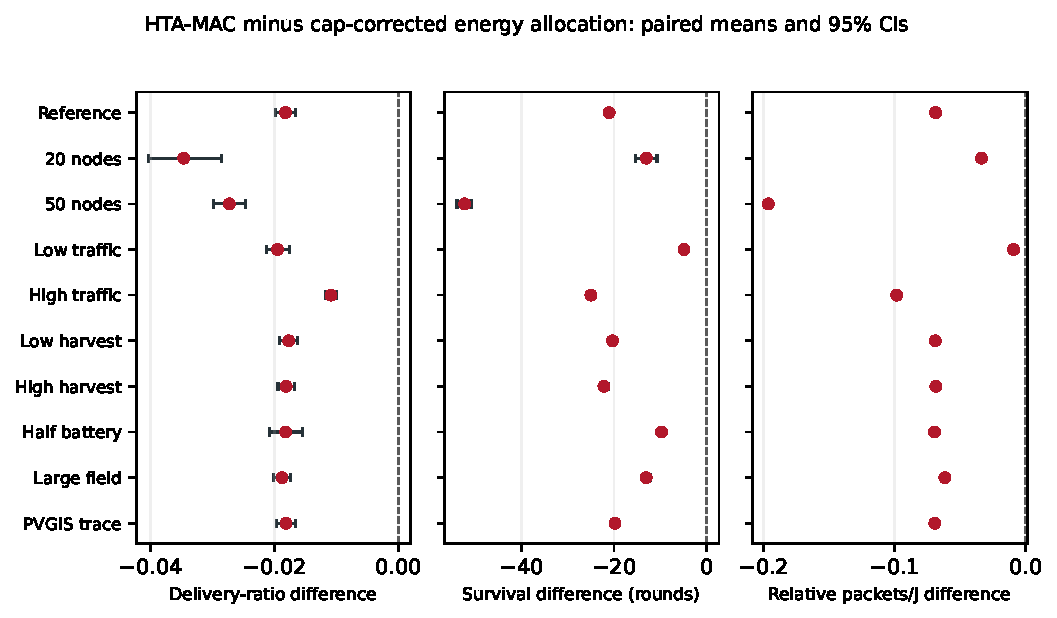
\includegraphics[width=0.96\textwidth]{robustness_multimetric.pdf}
  \caption{Post-confirmation corrective audit of \method{} relative to
  queue-cap-feasible energy-proportional allocation. Points are paired means
  over 20 opened runs and bars are 20,000-resample bootstrap 95\% confidence
  intervals; target ranks are averaged within run.}
  \label{fig:forest}
\end{figure*}

Table~\ref{tab:transfer} gives the corrected transfer matrix. The adverse
delivery sign persists under harvest scaling, half battery, a larger field, and
measured irradiance. Near-invariance across the low/high harvest interventions
indicates that, within the short pre-FND window and chosen energy scale, queue
and scheduled-role demand dominate the allocation difference. It should not be
interpreted as immunity to harvesting conditions.

\begin{table*}[t]
\centering
\caption{Transfer Matrix: \method{} Versus Energy-Proportional Allocation}
\label{tab:transfer}
\small
\begin{tabular}{@{}lrrrrrr@{}}
\toprule
& \multicolumn{3}{c}{Delivery ratio} & \multicolumn{2}{c}{Survival rounds} & \method{} packets/J \\
\cmidrule(lr){2-4}\cmidrule(lr){5-6}
Condition & \method & Baseline & Difference & \method & Baseline &  \\
\midrule
Reference (100) & 0.42770 & 0.44591 & -0.01821 & 128.28 & 149.32 & 225.77 \\
20 nodes & 0.90098 & 0.93562 & -0.03463 & 150.45 & 163.45 & 322.25 \\
50 nodes & 0.37523 & 0.40249 & -0.02726 & 118.25 & 170.48 & 212.27 \\
Low traffic & 0.87002 & 0.88951 & -0.01948 & 146.76 & 151.63 & 159.08 \\
High traffic & 0.29338 & 0.30424 & -0.01086 & 125.07 & 150.05 & 239.76 \\
Low harvest & 0.42854 & 0.44622 & -0.01768 & 125.60 & 145.91 & 225.78 \\
High harvest & 0.42761 & 0.44571 & -0.01810 & 130.99 & 153.16 & 225.84 \\
Half battery & 0.43513 & 0.45332 & -0.01819 & 62.86 & 72.60 & 224.64 \\
Large field & 0.43000 & 0.44876 & -0.01876 & 106.41 & 119.46 & 202.53 \\
PVGIS trace & 0.42831 & 0.44644 & -0.01813 & 124.54 & 144.31 & 225.71 \\
\bottomrule
\end{tabular}
\end{table*}

\subsection{Node-Count Scalability}

Fig.~\ref{fig:scalability} reports node-count evaluation from 50 to 300 nodes.
The shared-weight architecture is applied at each network size with a constant
116,033-parameter model, while the deterministic normalized budget $B/N$
reflects the evaluated node count. The energy comparator obeys the same queue
caps as the learned and constrained policies throughout this analysis.

Against energy-proportional allocation, \method{} has lower delivery at every
size: paired differences contract from $-0.0273$ (95\% CI $-0.0298$ to
$-0.0246$) at 50 nodes to $-0.0104$ ($-0.0111$ to $-0.0098$) at 300; all six
Holm-adjusted two-sided signed-rank values are $1.14\times10^{-5}$. Survival and
packets/J are also lower, but their deficits contract from $-52.23$ to $-6.95$
rounds and from $-19.63\%$ to $-2.56\%$, respectively. Conversely, from 100
through 300 nodes, \method{} lowers stale loss and raises fairness relative to
the heuristic; at 300 nodes the differences are $0.0252$ less stale loss and
$0.1345$ greater Jain fairness. The online primal--dual policy is stronger
overall: at 300 nodes it exceeds \method{} by 0.00585 delivery, 0.647 survival
rounds, 0.928\% packets/J, 0.00815 stale ratio, and 0.0559 fairness. Thus the
extension establishes executable scaling and a fairness--staleness tradeoff,
not performance dominance.

\begin{figure*}[t]
  \centering
  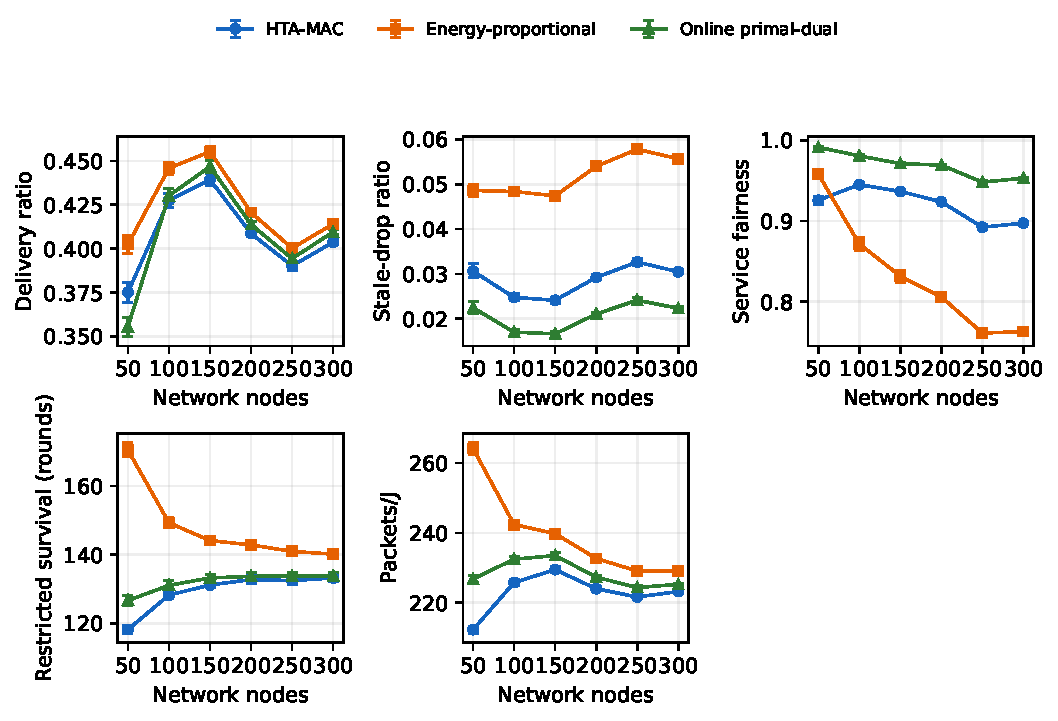
\includegraphics[width=0.92\textwidth]{scalability_performance.pdf}
  \caption{Node-count evaluation under a 24-slot cluster budget. Points are
  means over 20 paired runs and bars are 20,000-resample bootstrap 95\%
  confidence intervals. Every FND event was observed.}
  \label{fig:scalability}
\end{figure*}

\subsection{Network-Wide Load-Retention Probe}

Table~\ref{tab:lrfer} reports the simultaneous-all-cluster development probe.
\method{} retains 0.9561 of reference JWGE under high traffic, compared with
0.9274 for online primal--dual. The paired mean retention difference is 0.0287
(pilot bootstrap 95\% CI 0.01--0.05). With only five pairs, the exact two-sided
signed-rank value is $p=0.0625$; no confirmatory significance claim is made.
The energy-proportional pilot row is excluded because it used the subsequently
invalidated uncapped helper.

\begin{table}[t]
\centering
\caption{Exploratory Simultaneous-All-Cluster Fair-Energy Retention}
\label{tab:lrfer}
\scriptsize
\begin{tabular}{@{}lrrr@{}}
\toprule
Policy & Ref. JWGE & High-load JWGE & LRFER \\
\midrule
\method & 338.97 & 324.05 & \textbf{0.9561} \\
No CH context & 342.24 & 326.53 & 0.9541 \\
No set context & 346.56 & 327.43 & 0.9449 \\
Online primal--dual & 329.84 & 305.93 & 0.9274 \\
\bottomrule
\end{tabular}
\end{table}

The ordering is narrow rather than universal. \method{} is not distinguishable
from the no-CH-context intervention, and the pilot remains exploratory. LRFER
isolates resistance to traffic stress; it does not imply absolute service,
efficiency, or lifetime dominance.

\subsection{Corrected Pareto Interpretation}

The cap correction changes the earlier 20-node interpretation. At 20 nodes,
energy-proportional reaches 0.93562 delivery and 163.45 survival rounds, versus
0.90098 and 150.45 for \method{}. At the 100-node reference it likewise reaches
0.44591 and 149.32, versus 0.42770 and 128.28. Thus the heuristic lies above and
to the right of \method{} in both panels of Fig.~\ref{fig:pareto}. The learned
policy's remaining benefit is not Pareto superiority but its lower stale loss
and, except at the smallest sizes, higher service fairness.

\begin{figure}[t]
  \centering
  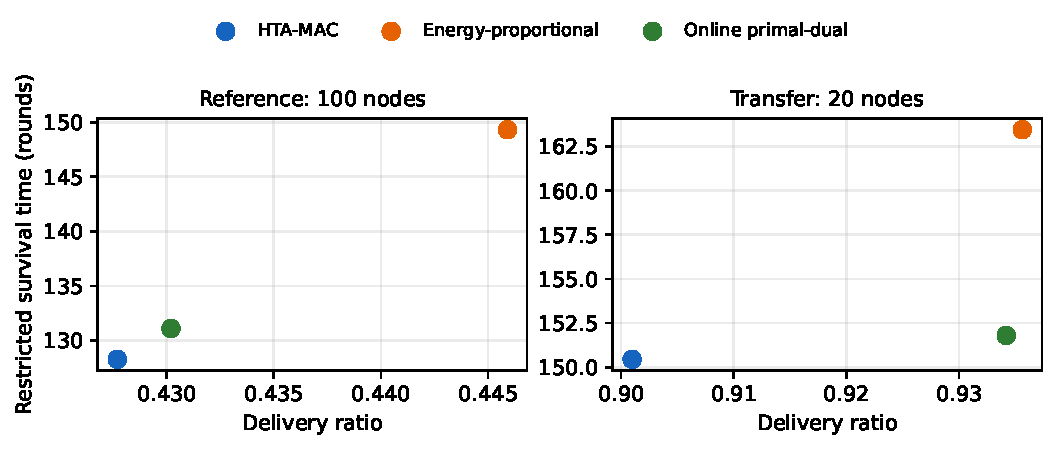
\includegraphics[width=\columnwidth]{reference_nodes20_pareto.pdf}
  \caption{Delivery--survival operating points in the reference and 20-node
  scenarios. Values are means over the 20 paired evaluation runs.}
  \label{fig:pareto}
\end{figure}

\subsection{Comparison with Online Primal--Dual Control}

Primal--dual is numerically better in the reference scenario: \method{} minus
the baseline is $-0.00250$ delivery (95\% CI $-0.00323$ to $-0.00174$),
$-2.82$ survival rounds (95\% CI $-3.43$ to $-2.14$), and $-2.876$\%
packets/J (95\% CI $-2.960$\% to $-2.797$\%). These differences are detectable
and the policies are not equivalent.

All three lower bounds nevertheless exceed the predefined non-inferiority margins:
$-0.00323>-0.01$, $-3.43>-6$, and $-2.960\%>-5\%$. \method{} is therefore
non-inferior within the declared practical tolerances. This result matters for
interpretation: the neural policy generalizes across the transfer matrix, but
the online constrained controller remains the stronger reference operating
point and should not be replaced solely on mean performance.

\begin{table}[t]
\centering
\caption{Reference Non-Inferiority to Online Primal--Dual}
\label{tab:noninferiority}
\scriptsize
\begin{tabular}{@{}lrrrl@{}}
\toprule
Metric & Difference & 95\% CI & Margin & Decision \\
\midrule
Delivery & $-0.00250$ & $[-0.00323,-0.00174]$ & $-0.01$ & Pass \\
Survival & $-2.82$ & $[-3.43,-2.14]$ & $-6$ & Pass \\
Packets/J & $-2.876\%$ & $[-2.960,-2.797]\%$ & $-5\%$ & Pass \\
\bottomrule
\end{tabular}
\end{table}

\subsection{QoS Floor and Model-Selection Ablation}

All policies satisfy the joint thresholds in every evaluation scenario.
The 100\% pass rate reveals that the binary floor is non-discriminative in this
matrix; it does not imply equal QoS. Continuous delivery, stale loss, fairness,
efficiency, and survival carry the comparison.

Two workload-conditioned extensions were examined as a development ablation.
A fully updated model passed the training QoS checks but reduced held-out
development delivery by 0.0027--0.0346 across six conditions. An adapter that
trained only new context parameters was stable but reduced delivery by
0.0094--0.0380. The simpler 65-feature controller was therefore selected before
final evaluation. The negative result suggests that aggregate workload context
alone does not resolve the high-load performance gap and may impair transfer.

A later matched optimization extension tested the full controller, removal of CH
context, removal of each auxiliary loss, and removal of both losses across
three optimizer initializations. All 15 lineages completed, but none passed the
predeclared convergence gate and four collapsed to all-sleep. Removing
concavity increased collapse from one of three full lineages to two of three;
removing both auxiliary losses prevented literal collapse but did not produce
stable QoS. These checkpoints are excluded from final inference. Consequently,
the study supports neither a causal component ranking nor selection of the
least-bad optimizer seed.

Fig.~\ref{fig:ablation} joins the two admissible ablation views. In the
same-checkpoint intervention, \method{} minus no-CH-context LRFER is 0.0020
(95\% CI $-0.0148$ to 0.0210, $p=1.0$), and the difference from no-set-context
is 0.0112 ($-0.0038$ to 0.0220, $p=0.1875$). Neither isolates a necessary
component. The optimization panel shows why no stronger attribution is made:
gate passes are 0/3 for every variant, while all-sleep collapse counts are
1/3 for the full model, 1/3 without CH context, 0/3 without trajectory loss,
2/3 without concavity loss, and 0/3 without both auxiliary losses.

\begin{figure*}[t]
  \centering
  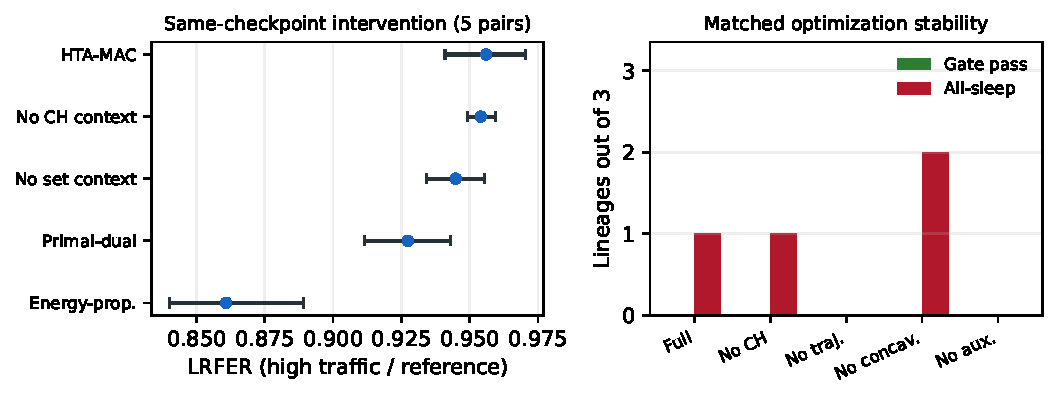
\includegraphics[width=0.92\textwidth]{ablation_evidence.pdf}
  \caption{Ablation evidence with explicit uncertainty and failure accounting.
  Left: exploratory five-pair LRFER means and bootstrap 95\% confidence
  intervals after same-checkpoint context interventions. Right: matched
  three-lineage optimization outcomes; zero-height green bars denote no gate
  passes, not missing observations.}
  \label{fig:ablation}
\end{figure*}

\section{Discussion}

\subsection{What the Results Establish}

The strongest evidence is now architectural and diagnostic rather than a
superiority effect. The shared set policy remains permutation equivariant,
exactly budget feasible, constant in learned parameter count, and executable
through 300 nodes. Empirically, its lower stale loss and
higher fairness from 100 nodes onward show that queue age and marginal slot
value alter who is served. They do not, however, compensate for the loss in
aggregate delivery, packets/J, or first-death survival.

The scaling evidence separates computational scalability from comparative
performance. Parameter storage is constant in branch capacity, hard feasibility
holds through 300 nodes, and isolated decision latency remains below 1~ms
through 100 active branches on the profiled CPU. From 100 to 300 nodes,
\method{} changes by only $-0.0240$ in delivery and $-1.14\%$ in packets/J,
while survival increases by 4.97 rounds. Nevertheless, the cap-corrected energy
heuristic retains higher delivery, survival, and packets/J, and online
primal--dual is slightly stronger overall. The model is therefore operationally
scalable to 300 nodes, but the experiment does not support comparative
dominance under a fixed 24-slot budget.

The network-wide probe adds a more specific hypothesis. Rather than claiming
the largest absolute score in every regime, \method{} loses the smallest
fraction of Jain-weighted goodput/J when traffic rises. This interpretation is
consistent with adaptive queue-age service, but remains exploratory because
the metric was derived from five development realizations. Its components and
the adverse FND effect remain load-bearing parts of the result.

The corrected lifetime result is sign-stable against the energy heuristic:
\method{} reaches FND earlier in all ten audited conditions. Packets/J is also
lower, so this is not merely a disagreement between average efficiency and a
tail lifetime metric. The likely mechanism remains scheduled-CH exposure, but
claiming an advantage will require a materially improved and newly validated
policy rather than a different composite metric.

The comparison with related papers must preserve simulator boundaries. The
11.79\% throughput improvement reported by Hasani \emph{et al.}
\cite{hasani2025drl}, the lifetime gains reported for underwater TDMA-RL
\cite{eris2024underwaterrl}, and HENO-MAC's delay reductions
\cite{sarang2024henomac} use different channels, energy assumptions, traffic,
and endpoints. They establish relevance, not a numerical leaderboard. Relative
to those evaluations, the present study adds paired uncertainty, multiplicity
control, exact budget enforcement, and a ten-condition transfer matrix; it is
weaker in physical validation and, compared with end-to-end protocols, in
network-layer scope.

\subsection{Limitations}

First, the network is simulated. PVGIS replay contributes a measured
irradiance trajectory but does not validate packet loss, radio energy, or
hardware timing. Second, the CH schedule is exogenous and balanced in
evaluation. Results do not show that jointly learning CH selection, routing,
and MAC would preserve the same effects. Third, the confirmatory experiment
intervenes on one scheduled cluster per rank rollout. Simultaneous network-wide
deployment has only five development realizations; it demonstrates executable
coupling but cannot support a final population claim.

Fourth, the thermal HMM is a fixed synthetic auxiliary, not a learned thermal
model. Fifth, the first deaths occur early relative to the 3000-round cap. All
events are observed, which simplifies survival estimation, but the experiment
does not characterize HND, LND, or long-run energy-neutral operation. Sixth,
the QoS floor is too permissive to discriminate the final policies. Finally,
the primal--dual baseline is numerically superior in the reference profile.
Non-inferiority within margins does not erase that difference. LRFER was
formulated after inspecting the development pilot, and the matched optimization
ablation failed all convergence gates; neither result may be used to select a
checkpoint or claim post-hoc superiority.

\subsection{Next Validation Step}

The immediate next experiment must repair categorical-head initialization and
QoS multiplier geometry, then pass a small multi-seed stability gate before
additional full training. Only a gate-qualified controller should be applied
once to the unused simultaneous-all-cluster cohort to confirm or reject LRFER,
extend survival endpoints to HND and LND, and test the calibrated QoS surface.
The highest-value independent validation is a separate simulator or a small
hardware-in-the-loop cluster driven by measured harvesting and current traces.
Only after that evidence should end-to-end co-optimization of CH rotation and
MAC be considered.

\section{Conclusion}

\method{} converts a combinatorial per-member TDMA decision into a
permutation-equivariant distributional branching policy with exact budget
projection and branch-capacity-independent parameter storage. The architecture
executes through 300 nodes and keeps absolute performance
reasonably stable from 100 to 300 nodes. However, a corrective post-confirmation
audit shows that queue-cap-feasible energy allocation has higher delivery,
survival, and packets/J in all ten tested conditions; online primal--dual is
also slightly stronger overall. \method{} instead lowers stale loss and, from
100 nodes onward, improves fairness relative to the energy heuristic. The
defensible contribution is therefore a scalable constrained architecture and
an honestly measured allocation tradeoff, not a publishable superiority claim.
A separate network-wide pilot suggests load-robust fair-energy retention, but
that post-development hypothesis and the failed optimization ablation require a
new, gate-qualified model and an untouched validation cohort.

\section*{Data Availability}

Model parameters, simulator specification, run-level results, statistical
analysis, and plotting materials are available in the accompanying
reproducibility archive.

% IEEE-formatted bibliography is embedded so this manuscript is self-contained.
\begin{thebibliography}{10}
\providecommand{\url}[1]{#1}
\csname url@samestyle\endcsname
\providecommand{\newblock}{\relax}
\providecommand{\bibinfo}[2]{#2}
\providecommand{\BIBentrySTDinterwordspacing}{\spaceskip=0pt\relax}
\providecommand{\BIBentryALTinterwordstretchfactor}{4}
\providecommand{\BIBentryALTinterwordspacing}{\spaceskip=\fontdimen2\font plus
\BIBentryALTinterwordstretchfactor\fontdimen3\font minus
  \fontdimen4\font\relax}

\bibitem{iannello2012ehmac}
F.~Iannello, O.~Simeone, and U.~Spagnolini, ``Medium access control protocols
  for wireless sensor networks with energy harvesting,'' \emph{IEEE
  Transactions on Communications}, vol.~60, no.~5, pp. 1381--1395, 2012.

\bibitem{gong2021ffss}
S.~Gong, X.~Liu, K.~Zheng, W.~Lu, and Y.-h. Zhu, ``TDMA scheduling schemes
  targeting high channel utilization for energy-harvesting wireless sensor
  networks,'' \emph{IET Communications}, 2021.

\bibitem{movva2022s2a2mac}
P.~Movva, K.~K. Kamarajugadda, and T.~R. Polipalli, ``An energy aware
  cluster-based routing and adaptive semi-synchronized MAC for energy
  harvesting WSN,'' \emph{International Journal of Communication Systems},
  2022.

\bibitem{sarang2024henomac}
S.~Sarang, G.~M. Stojanovi{\'c}, M.~Drieberg, V.~Jeoti, and M.~Valkama,
  ``HENO-MAC: Hybrid energy harvesting-based energy neutral operation MAC
  protocol for delay-sensitive IoT applications,'' in \emph{IEEE Wireless
  Communications and Networking Conference}, 2024.

\bibitem{lee2021reemac}
S.-B. Lee, J.-H. Kwon, and E.-J. Kim, ``Residual energy estimation-based MAC
  protocol for wireless powered sensor networks,'' \emph{Sensors}, vol.~21,
  no.~22, p. 7617, 2021.

\bibitem{sefuba2015adaptive}
M.~Sefuba, T.~Walingo, and F.~Takawira, ``Energy efficient medium access
  control protocol for clustered wireless sensor networks with adaptive
  cross-layer scheduling,'' \emph{Sensors}, vol.~15, no.~9, pp.
  24\,026--24\,053, 2015.

\bibitem{ge2021cooperative}
Y.~Ge, Y.~Nan, and X.~Guo, ``Maximizing network throughput by cooperative
  reinforcement learning in clustered solar-powered wireless sensor networks,''
  \emph{International Journal of Distributed Sensor Networks}, 2021.

\bibitem{hasani2025drl}
Z.~Hasani, M.~Mahdavimoghadam, R.~Mohammadi, Z.~Shirmohammadi, A.~Nikoofard,
  E.~Nikahd, and K.~Davoodi, ``Deep reinforcement learning-based mechanism to
  improve the throughput of EH-WSNs,'' \emph{Scientific Reports}, vol.~15,
  2025.

\bibitem{chu2019multiaccess}
M.~Chu, H.~Li, X.~Liao, and S.~Cui, ``Reinforcement learning based multi-access
  control and battery prediction with energy harvesting in IoT systems,'' 2018.
  [Online]. Available: \url{https://arxiv.org/abs/1805.05929}

\bibitem{sharma2019structure}
N.~Sharma, N.~Mastronarde, and J.~Chakareski, ``Accelerated structure-aware
  reinforcement learning for delay-sensitive energy harvesting wireless
  sensors,'' 2018. [Online]. Available: \url{https://arxiv.org/abs/1807.08315}

\bibitem{eris2024underwaterrl}
{\c{C}}.~Eri{\c{s}}, {\"O}.~M. G{\"u}l, and P.~Sar{\i}saray~B{\"o}l{\"u}k, ``A
  novel medium access policy based on reinforcement learning in
  energy-harvesting underwater sensor networks,'' \emph{Sensors}, vol.~24,
  no.~17, p. 5791, 2024.

\bibitem{zou2016predictive}
T.~Zou, S.~Lin, Q.~Feng, and Y.~Chen, ``Energy-efficient control with
  harvesting predictions for solar-powered wireless sensor networks,''
  \emph{Sensors}, vol.~16, no.~1, p.~53, 2016.

\bibitem{meshkati2007energy}
F.~Meshkati, H.~V. Poor, S.~C. Schwartz, and R.~V. Balan, ``Energy efficiency
  and delay quality-of-service in wireless networks,'' 2007. [Online].
  Available: \url{https://arxiv.org/abs/cs/0601098}

\bibitem{gao2017statistical}
Y.~Gao, W.~Cheng, and H.~Zhang, ``Statistical-QoS guaranteed energy efficiency
  optimization for energy harvesting wireless sensor networks,''
  \emph{Sensors}, vol.~17, no.~9, p. 1933, 2017.

\bibitem{yang2018fairness}
Z.~Yang, W.~Xu, Y.~Pan, C.~Pan, and M.~Chen, ``Optimal fairness-aware time and
  power allocation in wireless powered communication networks,'' \emph{IEEE
  Transactions on Communications}, vol.~66, no.~7, pp. 3122--3135, 2018.

\bibitem{jain1984fairness}
R.~Jain, D.-M. Chiu, and W.~R. Hawe, ``A quantitative measure of fairness and
  discrimination for resource allocation in shared computer systems,''
  \emph{DEC Research Report TR-301}, 1984.

\bibitem{jaffres2010multiobjective}
K.~Jaffr{\`e}s-Runser, C.~Comaniciu, and J.-M. Gorce, ``A multiobjective
  optimization framework for routing in wireless ad hoc networks,'' 2010.
  [Online]. Available: \url{https://arxiv.org/abs/0902.0782}

\bibitem{li2018fair}
K.~Li, C.~Yuen, B.~Kusy, R.~Jurdak, A.~Ignjatovic, S.~S. Kanhere, and S.~Jha,
  ``Fair scheduling for data collection in mobile sensor networks with energy
  harvesting,'' 2016. [Online]. Available:
  \url{https://arxiv.org/abs/1603.02476}

\bibitem{biason2016decentralized}
A.~Biason, S.~Dey, and M.~Zorzi, ``A decentralized optimization framework for
  energy harvesting devices,'' 2017. [Online]. Available:
  \url{https://arxiv.org/abs/1701.02081}

\bibitem{leong2020drl}
A.~S. Leong, A.~Ramaswamy, D.~E. Quevedo, H.~Karl, and L.~Shi, ``Deep
  reinforcement learning for wireless sensor scheduling in cyber-physical
  systems,'' 2018. [Online]. Available: \url{https://arxiv.org/abs/1809.05149}

\bibitem{bellemare2017c51}
M.~G. Bellemare, W.~Dabney, and R.~Munos, ``A distributional perspective on
  reinforcement learning,'' \emph{Proceedings of Machine Learning Research},
  vol.~70, pp. 449--458, 2017.

\bibitem{tavakoli2018branching}
A.~Tavakoli, F.~Pardo, and P.~Kormushev, ``Action branching architectures for
  deep reinforcement learning,'' in \emph{Proceedings of the AAAI Conference on
  Artificial Intelligence}, vol.~32, no.~1, 2018.

\bibitem{zaheer2017deepsets}
M.~Zaheer, S.~Kottur, S.~Ravanbakhsh, B.~P{\'o}czos, R.~Salakhutdinov, and
  A.~J. Smola, ``Deep sets,'' in \emph{Advances in Neural Information
  Processing Systems}, vol.~30, 2017.

\bibitem{heinzelman2000leach}
W.~R. Heinzelman, A.~Chandrakasan, and H.~Balakrishnan, ``Energy-efficient
  communication protocol for wireless microsensor networks,'' in
  \emph{Proceedings of the 33rd Hawaii International Conference on System
  Sciences}, 2000.

\bibitem{uno2014rmst}
H.~Uno, B.~Claggett, L.~Tian, E.~Inoue, P.~Gallo, T.~Miyata, D.~Schrag,
  M.~Takeuchi, Y.~Uyama, L.~Zhao, H.~Skali, S.~Solomon, S.~Jacobus, M.~Hughes,
  M.~Packer, and L.-J. Wei, ``Moving beyond the hazard ratio in quantifying the
  between-group difference in survival analysis,'' \emph{Journal of Clinical
  Oncology}, vol.~32, no.~22, pp. 2380--2385, 2014.

\bibitem{altman1999cmdp}
E.~Altman, \emph{Constrained Markov Decision Processes}. Chapman and Hall/CRC,
  1999.

\bibitem{pvgis2020}
{European Commission Joint Research Centre}, ``Photovoltaic geographical
  information system (PVGIS) ERA5 hourly radiation data,'' 2020.

\bibitem{efron1994bootstrap}
B.~Efron and R.~J. Tibshirani, \emph{An Introduction to the Bootstrap}.
  CRC Press, 1994.

\bibitem{wilcoxon1945}
F.~Wilcoxon, ``Individual comparisons by ranking methods,'' \emph{Biometrics
  Bulletin}, vol.~1, no.~6, pp. 80--83, 1945.

\bibitem{holm1979}
S.~Holm, ``A simple sequentially rejective multiple test procedure,''
  \emph{Scandinavian Journal of Statistics}, vol.~6, no.~2, pp. 65--70, 1979.

\end{thebibliography}

\end{document}
